% !TEX root = \linearpartition.tex

% state the problem
% RNA secondary structure prediction is a well-known problem, and it has been used for medical design. 
% Compared with MFE-based methods, partition function-based methods attract more and more attention due to their higher accuracy and ability to predict pseudoknots.
% Recently, 
% For example, almost every week a new ncRNA is found to be regulated in a particular disease, or a new class of noncoding
% transcripts is uncovered by a transcriptomic study, or a new
% article heralds a paradigm shift that lncRNAs will bring to
% our understanding of biology 
% Each year, noncoding RNA 
% Ribonucleic acid (RNA) 

\begin{figure*}[t]
\center
\begin{tabular}{cccc}
\panel{A} & \panel{B} & \panel{C} & \panel{D}\\[-0.4cm]
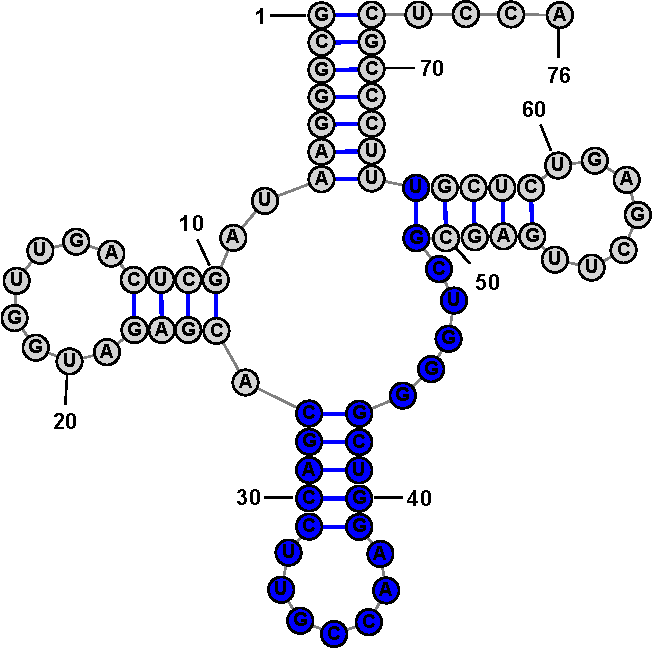
\includegraphics[scale=0.3]{figs/gold_RNAstructure}
&
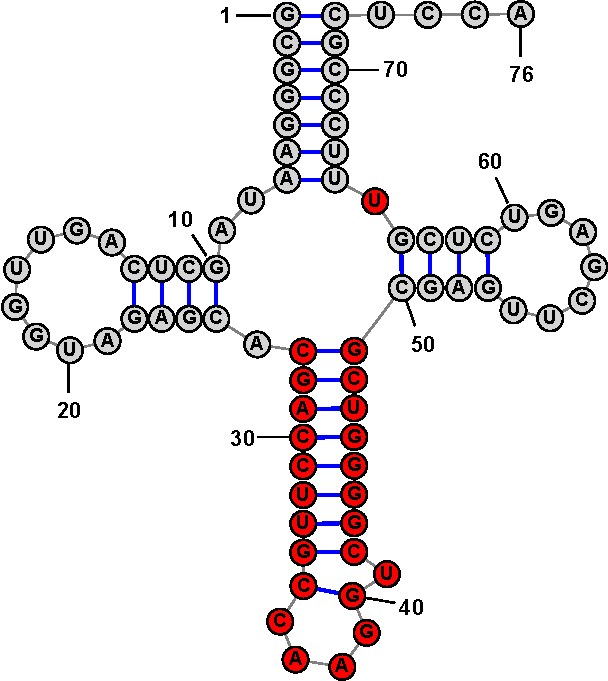
\includegraphics[scale=0.3]{figs/mfe_RNAstructure}
&
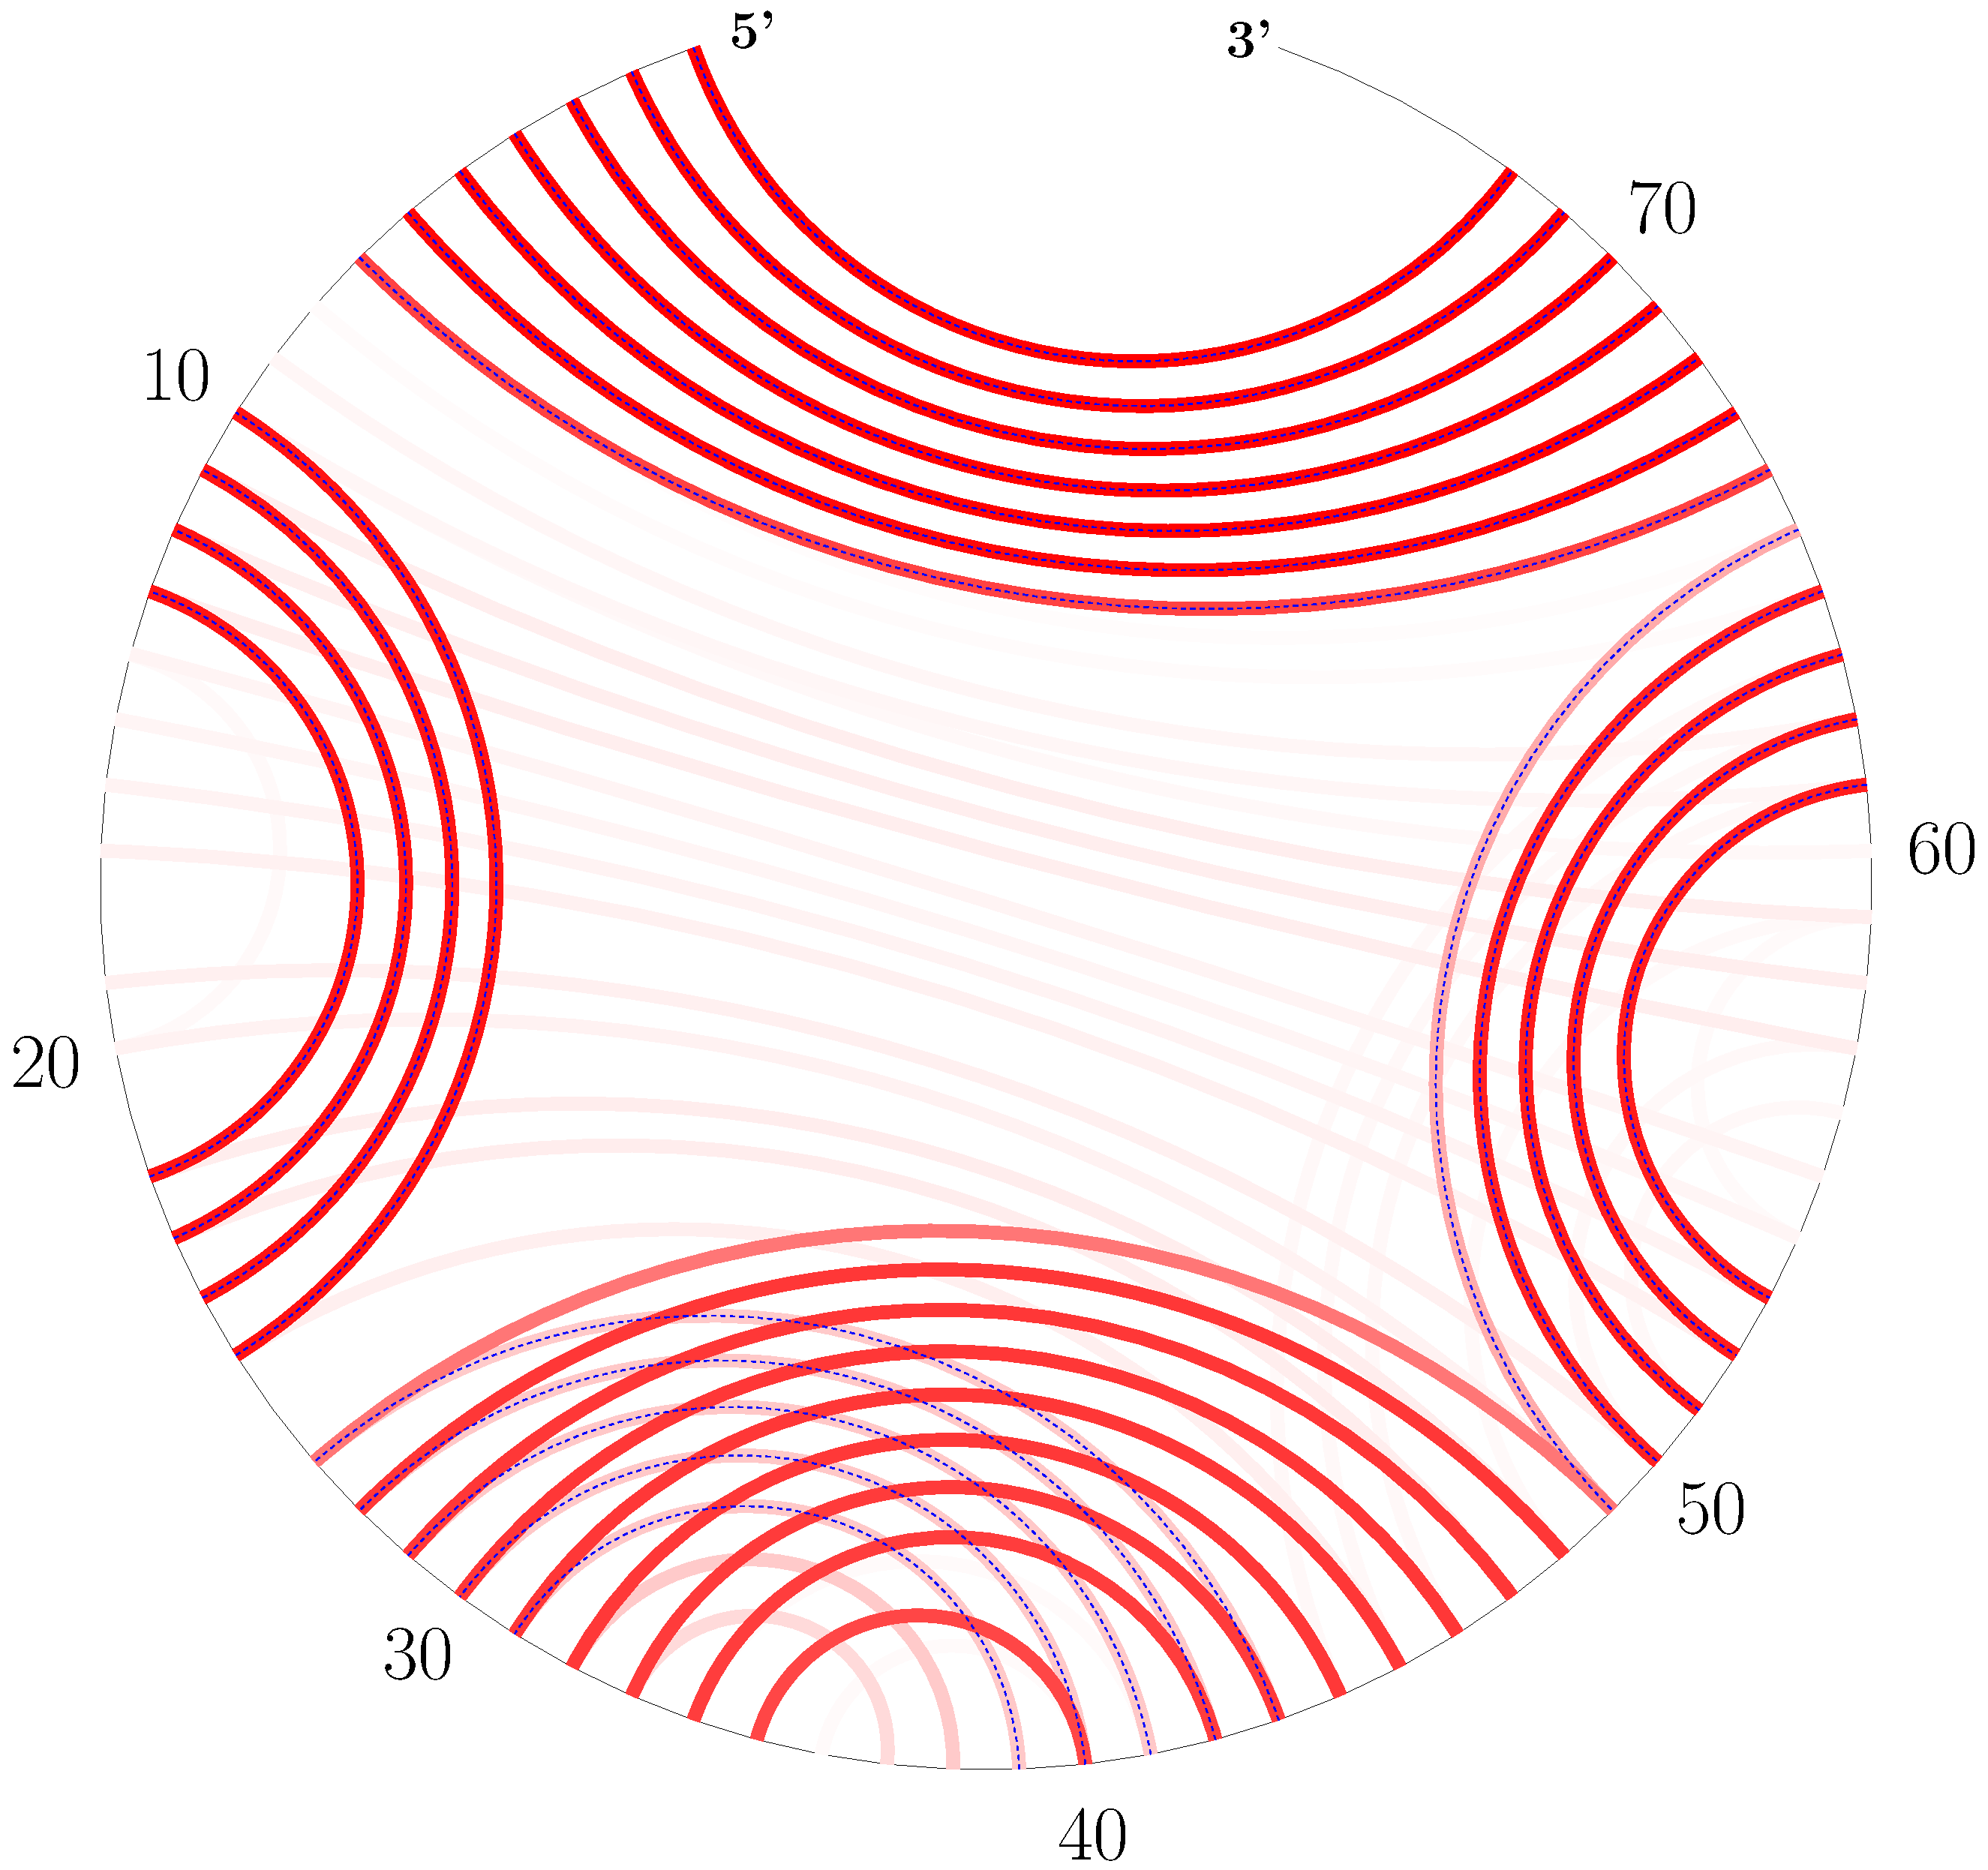
\includegraphics[scale=0.085]{figs/tRNA_circular}
&
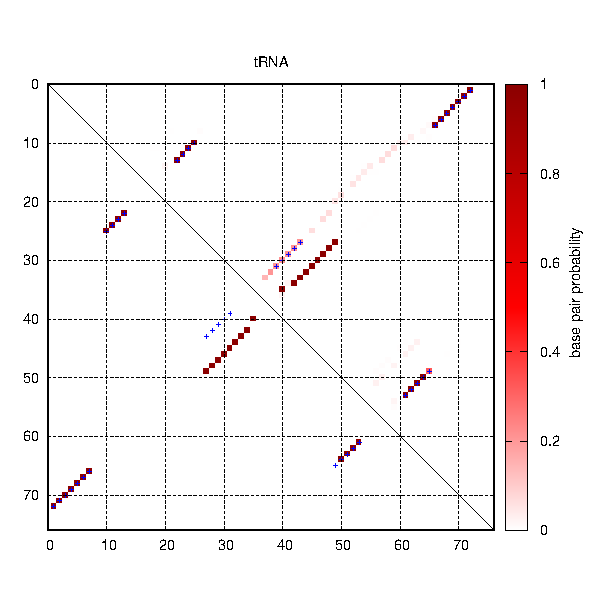
\includegraphics[scale=0.4]{figs/tRNA_heatmap_dark}

\end{tabular}
\caption{
Comparison of MFE-based method and partition function-based method. 
    {\bf A}: ground truth secondary structure of {\it E.~coli} tRNA$^\textit{Gly}$; 
    {\bf B}: the corresponding MFE structure. 
    Structural difference are denoted with blue in ground truth structure and red in MFE structure;
    {\bf C}: the corresponding circular representation.
    Ground truth base pairs are denoted with dash blue lines. 
    Base pair probabilities are denoted with red solid lines and line shade is proportional to probability value.
    {\bf D}: the corresponding heatmap representation.
    MFE structure (lower triangle) misses some ground truth base pairs (blue cross), 
    while base pair probability matrix (upper triangle) covers these correct base pairs. 
\label{tRNA}}
\end{figure*}

For past decades, our understanding of ribonucleic acid (RNA) is changing. 
New proofs reveal that noncoding RNAs (ncRNAs) are involved in multiple processes, such as controlling gene expression, guiding RNA modifications \cite{Eddy:2001}, or regulating a particular disease \cite{Kung+:2013}. 
These functionalities are highly related to RNA's structure, 
% but determining the structure using experimental methods is costly and time-comsuming. 
%%%%%%%%5
% from proposal
so being able to rapidly determine the structure is extremely useful 
given the overwhelming pace of increase in genomic data (about 1021 base-pairs per year \cite{stephens+:2015}) %[97] 
and given the small percentage of sequences that have experimentally determined structure. 
While experimental assays still constitute the most reliable way to determine structures, they are prohibitively costly, slow, and difficult.
% and therefore computational prediction provides an attractive alternative.
%%%%%%%%%%%%
% Due to such limitations, fast and accurate RNA structure prediction is required and desired,


Due to such limitations computational prediction is required and desired, however, predict full RNA structure is very challenging, even more difficult than protein folding \cite{mccaskill:1990}. 
Alternatively, RNA secondary structure, 
the double helices folding structure formed by self-complementary nucleotides (A-U, G-C, G-U base pairs) 
% in biologically active RNAs 
\cite{Tinoco+Bustamante:1999},
provides detailed information to help understand RNA's 
% mechanism of functionality
functionality 
\cite{tinoco+:1971},
and is a useful as a starting point to further predict full tertiary structure \cite{auron+:1982}.
Furthermore, nesting secondary structure prediction problem, though still challenging, is well-defined in mathematics formation, and can be suitable modeled with the summation of decomposable free energy. 
Utilizing this decomposable nature, 
cubic runtime dynamic programming algorithm 
for nesting secondary structure prediction are proposed \cite{nussinov+jacobson:1980}, 
followed by an important paradigm free energy minimization (MFE) method \cite{zuker+stiegler:1981} when a single structure is expected.
% and some prediction systems based on these algorithms, such as RNAstructure \cite{mathews+turner:2006}, \contrafold \cite{do+:2006} and \viennarnafold \cite{lorenz+:2011}, 
% have greatly improved the accuracy of prediction and are widely used.
% MEA -> partition function 
% For a given sequence, predicting the structure of minimum free energy (MFE) under certain free energy model by dynamic programming is a classical method for RNA secondary structure prediction. 
% cted.Free energy minimization is an important paradigm for predicting structure when a single structure is expe
% In the absence of many homologous sequences, the accuracy of MFE structure is 73\% in average \cite{mathews:2004}.
% However, this method assumes all thermodynamic parameters are correct and the energy model is perfect, which are both no the case in reality.
% Also, this method neglects the facts that multiple conformations exits at equilibrium \cite{mathews:2004}.
This method gives a practical solution to predict secondary structure, however, it neglects the facts that multiple conformations exit at equilibrium \cite{mathews:2004}, as well as abandons all pseudoknotted structures.
Many RNA sequences, for example mRNAs, exist in a thermodynamic ensemble of structures 
\cite{lai+:2018}.%[53].



% As an alternative, partition function-based method \cite{mccaskill:1990} provides an ensemble of all pseudoknot-free structures, and based on it base pair probabilities and structural entropy \cite{Huynen+} can be calculated.  
As an alternative, partition function-based method provides a normalization factor from which we can estimate base pairing probabilities 
\cite{mccaskill:1990, mathews:2004}% [75, 66]
 or statistically sample structures from the ensemble 
 \cite{ding+:2005, mathews:2006}% [25, 70].
% In this way not only one single structure but a distribution of base pair probability is available, which is more suitable to simulate RNA conformations at equilibrium. 
The base pairing probabilities also provide confidence estimates for predicted pairs 
\cite{mathews:2004, Zuber+:2018}% [66, 123]. 
As a by-product, the pair probabilities also enable maximum expected accuracy (MEA) structure prediction 
\cite{do+:2006, lu+:2009}% [29, 62].
Moreover, although partition function-based method excluded pseudoknotted structures during dynamic programming process, 
it is able to predict pseudoknotted base pairs and structure by using pair probability matrix, and pseudoknotted prediction systems such as HotKnot \cite{Ren+:2005}, ProbKnot \cite{bellaousov+mathews:2010}, DotKnot \cite{Sperschneider+Datta:2010} and IPknot \cite{Sato+:2011} all take pair probability matrix as inputs. 
Therefore, there has been a general shift from the classical MFE-based methods to partition function-based methods. 
Figure~\ref{tRNA} compares MFE-based and partition function-based methods.
% Furthermore, single structure prediction based on partition function calculation, such as maximum expected accuracy (MEA) ThreshKnot \cite{do+:2006, threshknot}, achieves higher accuracy in average. 

% speed
However, this partition function-based method, 
as well as prediction systems based on it such as RNAstructure \cite{mathews+turner:2006}, \contrafold \cite{do+:2006} and \viennarnafold \cite{lorenz+:2011}, 
suffers the slowness from its $O(n^3)$ runtime and scales poorly with longer sequences. 
Compared with $O(n^3)$ MFE-based method 
the slowness is even more severe.
% because function-based method takes two-round cubic loops for inside-outside calculation.
Recently, LinearFold \cite{Huang+:2019}, 
the first linear-time MFE-based (approximate) algorithm for RNA folding, 
achieves significant efficiency and scalability improvement and higher accuracy than classical $O(n^3)$ MFE-based method, especially on long sequence. 
Borrowed the efficient linearize idea from LinearFold, we presents \linearpartition, 
which approximates the partition function and base pair probability matrix in linear time, to address speed bottleneck in existing systems.
Similar as LinearFold, \linearpartition incrementally parses a RNA sequence using a left-to-right fashion dynamic programming, 
and further applys beam prune \cite{Huang+Sagae:2010} to narrow search space
 % with substructure of lower energy.
and only retain states with top $b$ lowest energy, where $b$ is the beam size.
Though introducing beam prune results to giving up some possible structures,
the well-designed pruning heuristic makes sure that only structures with worse energy are neglected,
and partition function is still similar as exact search.


\linearpartition, inherits LinearFold's efficiency and accuracy. \linearpartition is 10$\times$ faster than the baseline \viennarnafold for the longest sequence (about 3000 nucleotides) in the dataset. 
Not only fast, \linearpartition even leads to a small improvement in MEA and ProbKnot prediction using the probability matrix computed in linear time.
Surprisingly, \linearpartition achieves better accuracy on longer families (16S and 23S rRNA).


% \begin{itemize}
% \item Present an alternative left-to-right dynamic programming fashion for partition function calculation.
% \item The first algorithm to achieve linear runtime and space for partition function and base pair probability calculation.
% % \item . 
% \end{itemize}


